\documentclass{article}
\usepackage{amsmath}
\usepackage{amssymb}
\usepackage{graphicx}
\usepackage{hyperref}
\usepackage[version=4]{mhchem}


\begin{document}
\section*{Problem}
\(A B\) is the chord perpendicular to the diameter \(C D . O\) is the center. Find the length of \(O P\) if \(A P=4 \mathrm{~cm}\) and \(P D=2 \mathrm{~cm}\).\\
\centering
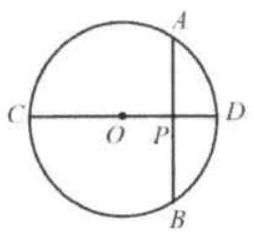
\includegraphics[width=\textwidth]{images/170(3).jpg}

\section*{Solution}
3 cm .\\
Connect \(A C\) and \(A D\).\\
Since \(C D\) is the diameter, \(\angle C A D=90^{\circ}\).\\
\(A P^{2}=C P \times P D \Rightarrow 4^{2}=(2 r-2) \times 2 \Rightarrow r=5\).\\
\(O P=5-2=3 \mathrm{~cm}\).\\
\centering
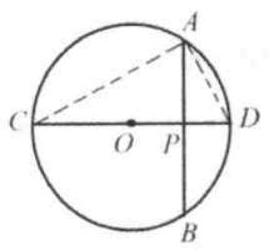
\includegraphics[width=\textwidth]{images/173(3).jpg}

\end{document}
